%%%%%%%%%%%%%%%%%%%%%%%%%%%%%%%%%%%%%%%%%%%%%%%%%%%%%%%%%%%%%%%%%%%%%%
% Template para artigos da SBC
% Adaptado para o trabalho prático de Processamento de Dados com Grafos
%%%%%%%%%%%%%%%%%%%%%%%%%%%%%%%%%%%%%%%%%%%%%%%%%%%%%%%%%%%%%%%%%%%%%%

\documentclass[12pt]{article}

\usepackage{sbc-template}
\usepackage{graphicx,url}
\usepackage[utf8]{inputenc}  
\usepackage{amsmath} % Para ambientes matemáticos
\usepackage{listings} % Para blocos de código
\usepackage{xcolor} % Para cores no código

% Configuração para blocos de código
\definecolor{codegreen}{rgb}{0,0.6,0}
\definecolor{codegray}{rgb}{0.5,0.5,0.5}
\definecolor{codepurple}{rgb}{0.58,0,0.82}
\definecolor{backcolour}{rgb}{0.95,0.95,0.92}

\lstdefinestyle{customStyle}{
    backgroundcolor=\color{backcolour},   
    commentstyle=\color{codegreen},
    keywordstyle=\color{magenta},
    numberstyle=\tiny\color{codegray},
    stringstyle=\color{codepurple},
    basicstyle=\ttfamily\footnotesize,
    breakatwhitespace=false,         
    breaklines=true,                 
    captionpos=b,                    
    keepspaces=true,                 
    numbers=left,                    
    numbersep=5pt,                  
    showspaces=false,                
    showstringspaces=false,
    showtabs=false,                  
    tabsize=2
}
\lstset{style=customStyle}
     
\sloppy

\title{Gestão de Dependências em Projetos Go com Ordenação Topológica}

% FAVOR PREENCHER OS DADOS DOS AUTORES E INSTITUIÇÕES
\author{Nicholas Pereira Cristófaro\inst{1}, Nome Sobrenome do Aluno 2\inst{1}}

\address{Pontifícia Universidade Católica de Minas Gerais\\
  Belo Horizonte -- Minas Gerais -- Brasil
  \email{nicholaspcr@gmail.com, email2@dominio.com}
}

\begin{document} 

\maketitle

\begin{resumo} 
  A complexidade crescente dos sistemas de software modernos exige mecanismos robustos para a gestão de dependências. Este artigo apresenta o desenvolvimento de uma ferramenta para análise e visualização de dependências em projetos na linguagem Go. O problema da ordem de inicialização de pacotes é modelado como um grafo direcionado, onde os pacotes são os vértices e as importações representam as arestas. Utilizando o algoritmo de Kahn para ordenação topológica, a ferramenta determina a sequência de compilação segura e identifica a existência de dependências cíclicas, um erro crítico em Go. O trabalho detalha a implementação em Python, desde a análise do código-fonte até a geração de uma visualização gráfica interativa do grafo, alinhando-se ao tema de gestão de conflitos em sistemas de dependência.
\end{resumo}

\begin{abstract}
  The growing complexity of modern software systems demands robust mechanisms for dependency management. This paper presents the development of a tool for analyzing and visualizing dependencies in projects written in the Go language. The package initialization order problem is modeled as a directed graph, where packages are vertices and imports represent edges. Using Kahn's algorithm for topological sorting, the tool determines the safe compilation sequence and identifies the existence of cyclic dependencies, a critical error in Go. The work details the Python implementation, from source code parsing to the generation of an interactive graphical visualization of the graph, aligning with the theme of conflict management in dependency systems.
\end{abstract}

\section{Informações Gerais}

O presente trabalho se insere no contexto do desenvolvimento de ferramentas computacionais para processamento de dados estruturados como grafos, com foco na aplicação de conceitos da teoria dos grafos e na adesão a boas práticas de engenharia de software. O objetivo central é apresentar uma solução para um problema prático na análise de projetos de software desenvolvidos na linguagem Go (Golang): a determinação da ordem de inicialização de seus pacotes. A linguagem Go, reconhecida por sua eficiência e robusto sistema de gerenciamento de pacotes, impõe uma ordem de inicialização determinística onde as dependências de um pacote são inicializadas antes do próprio pacote. Essa característica é crucial para a correta execução das funções `init()`, responsáveis pela configuração inicial de cada pacote.

A ordem de inicialização de pacotes em Go pode ser naturalmente modelada como um grafo de dependências direcionado acíclico (DAG). A obtenção de uma ordenação topológica deste grafo revela a sequência exata em que os pacotes são carregados e suas funções `init()` são executadas. Tal visualização não apenas auxilia na compreensão da arquitetura de um projeto, mas também é fundamental para ferramentas de análise estática e otimização de compilação. Para alcançar este objetivo, optou-se pela implementação do algoritmo de Kahn, uma abordagem clássica para a ordenação topológica. Este trabalho detalha o desenvolvimento de um script em Python que utiliza o algoritmo de Kahn para processar as dependências de um projeto Golang, gerando como saída a sua ordenação topológica. A ferramenta desenvolvida visa oferecer um mecanismo eficaz para que desenvolvedores e analistas possam visualizar e gerenciar a complexa rede de interdependências em seus projetos Go, contribuindo para uma melhor compreensão da sequência de inicialização e, consequentemente, do comportamento do software.

Os artigos completos devem respeitar os limites de página definidos pela conferência.
Conferências que publicam apenas resumos pedem por textos de \textbf{uma} página.

\section{Primeira Página} \label{sec:firstpage}

A primeira página deve exibir o título do artigo, o nome e o endereço dos
autores, o abstract em inglês e o resumo em português (resumos são
necessários apenas para artigos escritos em português). O título deve ser centralizado
em toda a página, em fonte negrito de 16 pontos e com 12 pontos de espaço
antes de si. Os nomes dos autores devem ser centralizados em fonte de 12 pontos, negrito, todos
dispostos na mesma linha, separados por vírgulas e com 12 pontos de
espaço após o título. Os endereços devem ser centralizados em fonte de 12 pontos, também com
12 pontos de espaço após os nomes dos autores. Os endereços de e-mail devem ser
escritos usando a fonte Courier New, tamanho nominal de 10 pontos, com 6 pontos de espaço
antes e 6 pontos de espaço depois. O abstract e o resumo (se for o caso) devem estar em fonte Times de 12 pontos,
com recuo de 0,8 cm em ambos os lados. A palavra \textbf{Abstract} e \textbf{Resumo},
deve ser escrita em negrito e preceder o texto.

\section{CD-ROMs e Anais Impressos}

Em algumas conferências, os artigos são publicados em CD-ROM enquanto apenas o
resumo é publicado nos Anais impressos. Neste caso, os autores são
convidados a preparar duas versões finais do artigo. Uma, completa, para ser
publicada no CD e a outra, contendo apenas a primeira página, com
abstract e resumo (para artigos em português).

\section{Seções e Parágrafos}

Os títulos das seções devem estar em negrito, 13pt, alinhados à esquerda. Deve haver um espaço extra
de 12 pt antes de cada título. A numeração das seções é opcional. O primeiro
parágrafo de cada seção não deve ser recuado, enquanto as primeiras linhas dos
parágrafos subsequentes devem ser recuadas em 1,27 cm.

\subsection{Subseções}

Os títulos das subseções devem estar em negrito, 12pt, alinhados à esquerda.

\section{Figuras e Legendas}\label{sec:figs}


As legendas de figuras e tabelas devem ser centralizadas se tiverem menos de uma linha
(Figura~\ref{fig:exampleFig1}), caso contrário, justificadas e recuadas em 0,8 cm em
ambas as margens, como mostrado na Figura~\ref{fig:exampleFig2}. A fonte da legenda deve
ser Helvetica, 10 pontos, negrito, com 6 pontos de espaço antes e depois de cada
legenda.

\begin{figure}[ht]
\centering
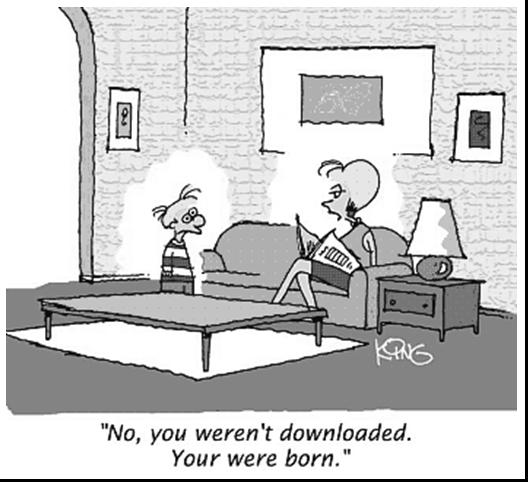
\includegraphics[width=.5\textwidth]{fig1.jpg}
\caption{Uma figura típica}
\label{fig:exampleFig1}
\end{figure}

\begin{figure}[ht]
\centering
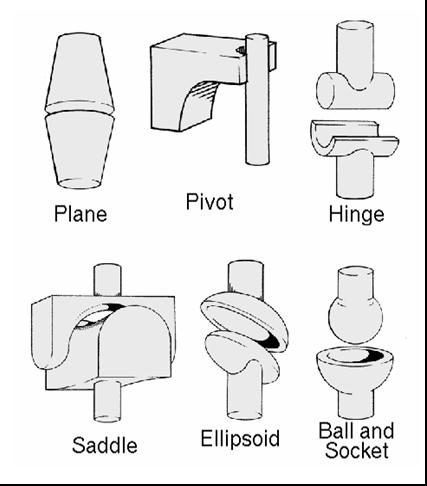
\includegraphics[width=.3\textwidth]{fig2.jpg}
\caption{Esta figura é um exemplo de uma legenda de figura que ocupa mais de uma
linha e é justificada considerando as margens mencionadas na Seção~\ref{sec:figs}.}
\label{fig:exampleFig2}
\end{figure}

Em tabelas, tente evitar o uso de fundos coloridos ou sombreados, e evite
linhas de enquadramento grossas, duplas ou desnecessárias. Ao relatar dados empíricos,
não use mais dígitos decimais do que o justificado por sua precisão e
reprodutibilidade. A legenda da tabela deve ser colocada antes da tabela (ver Tabela 1)
e a fonte usada também deve ser Helvetica, 10 pontos, negrito, com 6 pontos de
espaço antes e depois de cada legenda.

\begin{table}[ht]
\centering
\caption{Variáveis a serem consideradas na avaliação de técnicas de
interação}
\label{tab:exTable1}
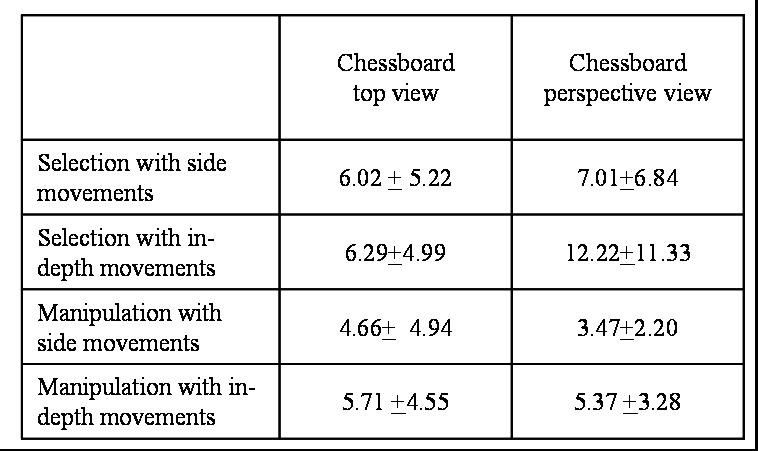
\includegraphics[width=.7\textwidth]{table.jpg}
\end{table}

\section{Imagens}

Todas as imagens e ilustrações devem ser em preto e branco, ou tons de cinza,
exceto para os artigos que estarão disponíveis eletronicamente (em CD-ROMs,
internet, etc.). A resolução da imagem no papel deve ser de cerca de 600 dpi para
imagens em preto e branco, e 150-300 dpi para imagens em tons de cinza. Não inclua
imagens com resolução excessiva, pois elas podem levar horas para imprimir, sem qualquer
diferença visível no resultado.

\section{Referências}

As referências bibliográficas devem ser inequívocas e uniformes. Recomendamos fornecer
as referências dos nomes dos autores entre colchetes, por exemplo, \cite{knuth:84},
\cite{boulic:91}, e \cite{smith:99}. As referências devem ser listadas usando fonte de tamanho 12, com 6 pontos de espaço
antes de cada referência. A primeira linha de cada referência não deve ser
recuada, enquanto as subsequentes devem ser recuadas em 0,5 cm.

\bibliographystyle{sbc}
\bibliography{sbc-template.bib}

\end{document}
